
\subsection[200 nm]{200 Nanometer Probe}
\begin{frame}
  \frametitle{Radiation resistance of D. Radiodurans (I)}

  \textit{D. Radiodurens} were cultured on a TEM grid and dried.  The
  locations of cells were registered under a light microscope and
  found again at APS beamline 2\,ID-D, where a 250\,nm
  probe was used.
  
  \begin{columns}
    \begin{column}{0.4\linewidth}
      \begin{center}
        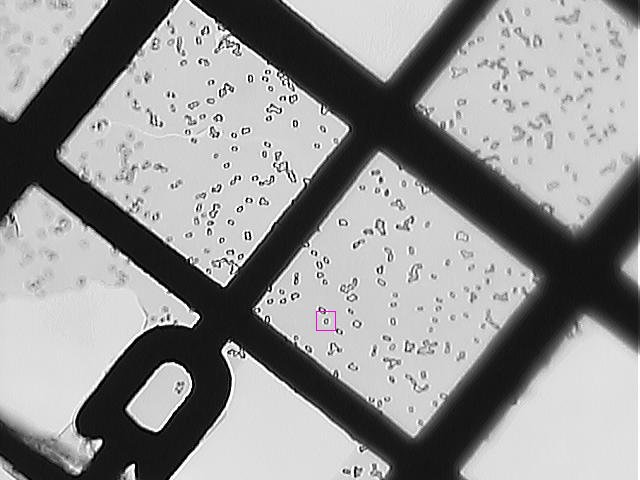
\includegraphics[width=0.8\linewidth]{xrf/dr_tem_grid.jpg}\\[1ex]
        {\tiny
          \begin{tabular}{ccc}
            element & max $\mu$g/cm$^2$ & max mass ppm \\
            \hline
            P  & 3.5200 & 312.3\\
            S  & 0.4790 & 42.5\\
            Cl & 0.2130 & 18.9\\
            K  & 2.3600 & 209.4\\
            Ca & 0.1300 & 11.5\\
            Cr & 0.0014 & 0.1\\
            Mn & 0.0155 & 1.4\\
            Fe & 0.0135 & 1.2\\
            Co & 0.0019 & 0.2\\
            Ni & 0.0024 & 0.2\\
            Cu & 0.0413 & 3.7\\
            Zn & 0.0457 & 4.1\\
          \end{tabular}
        }
      \end{center}
    \end{column}
    \begin{column}{0.6\linewidth}
      \begin{center}
        This proved to be a colony of four cells:\\[1ex]
        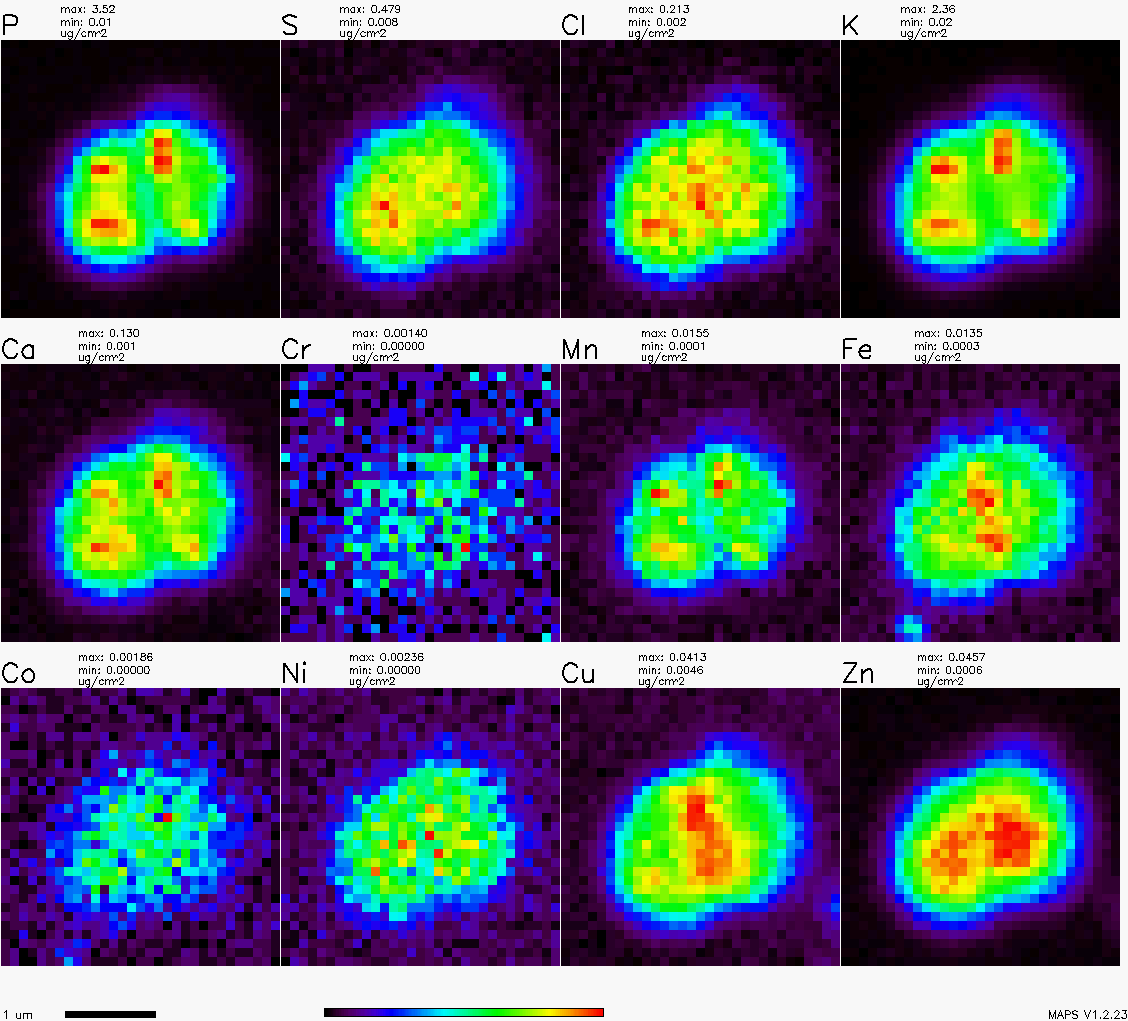
\includegraphics[width=0.9\linewidth]{xrf/dr_allmaps.png}
      \end{center}
    \end{column}
  \end{columns}

  \bigskip

  \begin{textblock*}{0.5\linewidth}(0pt,19\TPVertModule)
    \tiny M. Daly et el., \textit{Protein Oxidation Implicated as the
      Primary Determinant of Bacterial Radioresistance}, PLoS
    Biol \textbf{5}(4): e92 
    \href{http://dx.doi.org/10.1371/journal.pbio.0050092}
    {\color{Blue4}\texttt{doi:10.1371/journal.pbio.0050092}}
  \end{textblock*}
\end{frame}


\begin{frame}
  \frametitle{Radiation resistance of D. Radiodurans (II)}

  \textit{D. Radiodurens}:
  \begin{enumerate}
  \item is unusually resistent to high doses of ionizing radiation, even
    thriving under doses that would quickly kill other bacteria
  \item has high intracellular Mn/Fe concentration ratios compared to
    IR-sensitive bacteria
  \end{enumerate}

  \bigskip
  
  \begin{block}{We noticed a trend in the Fe and Mn distribution}
    \begin{itemize}
    \item Fe is enhanced in the cell walls.  It is available when
      needed for metabolism but sequestered from cell organs to
      protect them from Fenton chemistry.
    \item Mn in enhanced in cell body and is available to scavange
      radiolosis radicals near cell organs.
    \end{itemize}
  \end{block}

  \bigskip

  \begin{textblock*}{0.5\linewidth}(0pt,19\TPVertModule)
    \tiny M. Daly et el., \textit{Protein Oxidation Implicated as the
      Primary Determinant of Bacterial Radioresistance}, PLoS
    Biol \textbf{5}(4): e92
    \href{http://dx.doi.org/10.1371/journal.pbio.0050092}
    {\color{Blue4}\texttt{doi:10.1371/journal.pbio.0050092}}
  \end{textblock*}
\end{frame}

\begin{frame}
  \frametitle{Radiation resistance of D. Radiodurans (III)}

  Here are images we published on a diploid colony:

  \bigskip

  \begin{columns}
    \begin{column}{0.5\linewidth}
      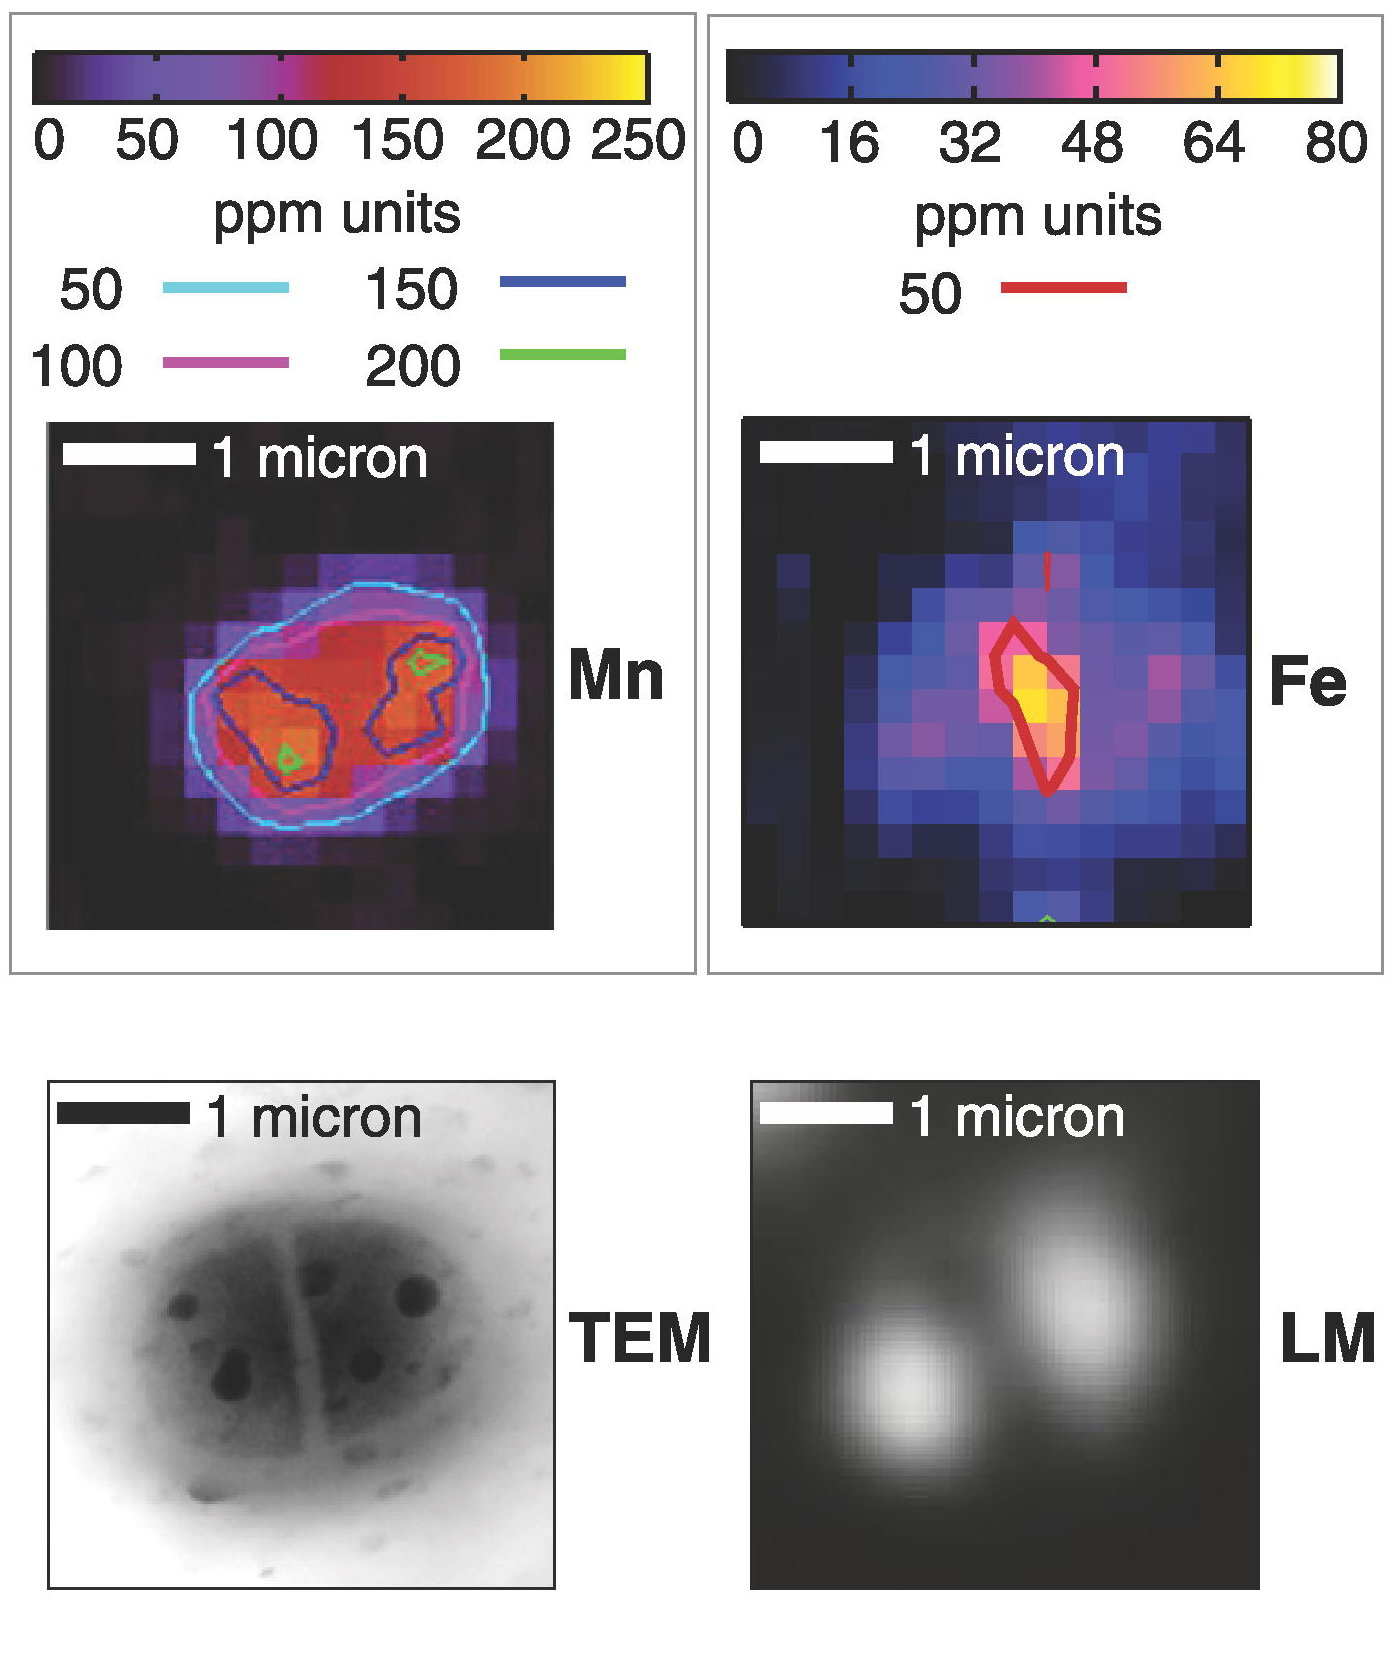
\includegraphics[width=\linewidth]{xrf/dr_4maps.jpg}
    \end{column}
    \begin{column}{0.5\linewidth}
      Superposing those four images:\\[1ex]
      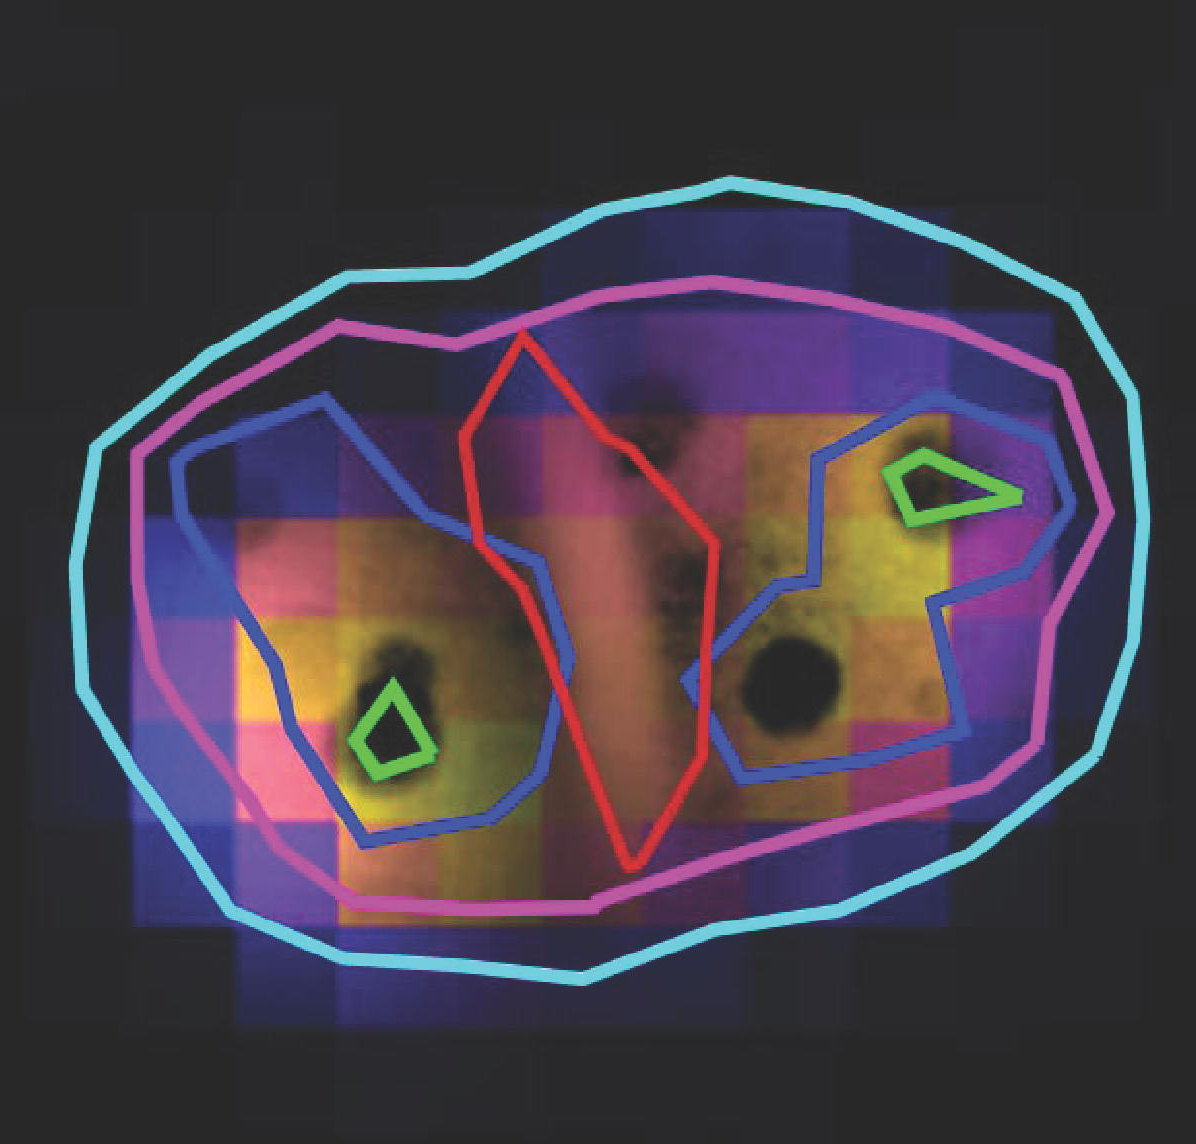
\includegraphics[width=\linewidth]{xrf/dr_superposed.jpg}
    \end{column}
  \end{columns}    
  
  \bigskip

  \begin{textblock*}{0.5\linewidth}(0pt,19\TPVertModule)
    \tiny M. Daly et el., \textit{Protein Oxidation Implicated as the
      Primary Determinant of Bacterial Radioresistance}, PLoS
    Biol \textbf{5}(4): e92
    \href{http://dx.doi.org/10.1371/journal.pbio.0050092}
    {\color{Blue4}\texttt{doi:10.1371/journal.pbio.0050092}}
  \end{textblock*}
\end{frame}

